\documentclass{article}   	                         % use "amsart" instead of "article" for AMSLaTeX format
\usepackage{fullpage}                		% ... or a4paper or a5paper or ... 
\usepackage{enumerate}				% Use enumerate to list subsections
\usepackage{graphicx}				% Use pdf, png, jpg, or eps§ with pdflatex; use eps in DVI mode
\usepackage{fancyvrb}
\usepackage{amsmath}
\usepackage{dsfont}
\newcommand{\ra}{\rightarrow}

%SetFonts

\title{Computer System Fundamentals HW \#2}
\author{Quan Zhou}
\date{Feb 10th, 2016 (update)}
\begin{document}
\maketitle
\section*{Problem 1}
\begin{enumerate}[(a)]
\item
N = 20; Pr(X) = 0.96; $Pr(\bar X)  = 1 - Pr(X) = 0.04$\\
so the event when 20 connections to the web server where no connections will be refused is a binomial distribution. Therefore we have: Pr(X = 20) = ${20 \choose 0} (Pr(X = 1))^{20}(Pr(X = 0))^0$ = 0.4420
\item
N = 20, $Pr(X = 19)$ = ${20 \choose 1} (Pr(X = 1))^{19}(Pr(X = 0))^1$ = 0.3683
\item
N = 20, $Pr(X > 17)$ = ${20 \choose 0} (Pr(X = 1))^{20}(Pr(X = 0))^0 + {20 \choose 1} (Pr(X = 1))^{19}(Pr(X = 0))^1 + {20 \choose 2} (Pr(X = 1))^{18}(Pr(X = 0))^2 + {20 \choose 3} (Pr(X = 1))^{17}(Pr(X = 0))^3$ = 0.9561
\item
$Pr(X \geq 4) = 1 - Pr(\bar X = 1) - Pr(\bar X = 2) - Pr(\bar X = 3) = 1 - 0.04 - (0.04)^2 - (0.04)^3= 0.9583$
\item
The event when some number of requests that will be successfully served before a connection is refused is geometric distribution. 
$\mathds{E}(X = 1)$ = $\frac{Pr(X)}{Pr(\bar X)}$ = $\frac{0.96}{0.04}$ = 24
\item
For the event of a sample size of 50 requests being processed through the web server, let's assume the distribution is Gaussian (Normal). so $\mathds{E}(X)$ = 50*0.96 = 48
\item
For a very large number of requests being processed through the web server, we could assume the number of successful requests through the server is normally distributed variable. Then we are able to find:\\
\begin{align*}
 z
 &\geq \frac{x - \mu}{\frac{\sigma}{\sqrt(n)}}
 \\& = \sqrt(50)(\frac{x}{\mu} - 1)(\frac{\mu}{\sigma})
 \\& = \sqrt(50)(\frac{x}{\mu} - 1)(\frac{\frac{1-p}{p}}{\frac{\sqrt(1-p)}{p}})
 \\& = \sqrt(50)(\frac{x}{\mu} - 1)(\sqrt(1-p))
 \\& = \sqrt(50)(\frac{0.95}{0.96} - 1)(\sqrt(0.96))
 \\& = -0.071
\end{align*}
By looking up the Z-table, we found the probability is 1- 0.4721  = 0.5278
\item
None. For all the questions are focused on what the odds are for successful or failing connection, and the variables are not function of time(for we assume the probability of successful or failing connection is constant or not a function of time). These questions have to do with availability of the web server, not reliability. Rather, if the questions were asked about the probability of the server is still up over a period of time, then it is a questions of reliability.\\

\end{enumerate}
\section*{Problem 2}
\begin{enumerate}[I]
\item
\begin{enumerate}[(a)]
\item
Since the arrival rate is 200 packets per second, so the parameter $\lambda$ = $\frac{200 packets}{second}\cdot \frac{10 second}{1000} $ = 2 . We have the following probability mass function (pmf) with Possion distribution:\\
\begin{center}
$f (x) = \left(\frac{2^x}{x!}\right)e^{-2}$\\
\end{center}
\item
The probability of more than 3 packets are received over the 10 msec period is given by the following equation:\\
\begin{align*}
 Pr (X > 3)
   & = 1 - Pr(X = 0) - Pr(X = 1) - Pr(X = 2) - Pr(X = 3)
 \\& = 1 - (1 + 2 + 2 + \frac{4}{3})e^{-2}
 \\& = 0.1429
\end{align*}
\item
Now the probability of inter-arrival time of packets is a exponentially distributed random variable. $\lambda$ is actually the rate of arrival packets at the Ethernet adapter, or 200 packet/msec, and we get:\\ 
\begin{center}
$g (T) = 200e^{-200T}$\\
\end{center}
\item
The probability of two packets will be separated by more than 8 msec is given by the cumulative distribution function (cdf) G:\\
\begin{center}
$G (T) = 1- e^{-0.2T}$\\
\end{center}
so:\\
\begin{align*}
 Pr (T > 8 msec)
   & = 1 - G(T = 8 msec)
 \\& = 1 - (1 - e^{-0.2T}
 \\& = e^{-1.6}
 \\& = 0.2019
\end{align*}
\item
The variance of an exponential distribution is given by $\lambda ^{-2}$, or standard deviation by $\lambda ^{-1}$, so we derive the standard deviation of the inter-arrival time of packet to be 5.
\end{enumerate}
\item
\begin{enumerate}[(a)]
\item
For one packet in the system, $T_s = 4.8 \text{  msec}$.  Therefore, the capacity this Ethernet Adapter is $\frac{1000}{4.8}$ or 208.33 packets per sec.
\item
Assuming the Ethernet adaptor is M/M/1 system (Poisson process arrival, exponential distribution for servicing and one server), the probability of having x packets in the system is given by:\\
\begin{equation}f(x) = (1-\rho)(\rho^x) = 0.04(0.96^x)\end{equation}
where the utilization $\rho =\lambda T_s = \frac{0.2} {\text{  msec}} 4.8 \text{  msec}  = 0.96$
\item
To find w, by Little's Law we have:\\
\begin{equation} w = \lambda T_w \end{equation} 
$T_w = T_q - T_s = 5 - 4.8 = 0.2 \text{  msec}$
Therefore:\\
$w = \lambda (0.2 \text{  msec}) = \frac{200 \text{   packets}}{1000 \text{   msec}} (0.2 \text{  msec}) = 0.04 \text{   packets}$
\item
As found from part (c), $T_w = 0.2 \text{  msec}$
\item
$\text{Slowdown} = \frac{1}{1-\rho} = \frac{1}{1- 0.96} =  \frac{1}{0.04} = 25$ 
\end{enumerate}

\end{enumerate}

\section*{Problem 3}
\begin{enumerate}[(a)]
\item
By definition, the exponential distribution has the following pdf:\\
\begin{equation} f(x) = \lambda e^{-\lambda x}\end{equation} 
In this problem, we will look at the inverse of above equation:\\
$y = \lambda e^{-\lambda x}$\\
$\frac{y}{\lambda} = e^{-\lambda x}$\\
$ln (\frac{y}{\lambda}) = -\lambda x $\\
$x = -\frac{ln (\frac{y}{\lambda})}{\lambda}$\\
Define $\frac{y}{\lambda}$ as a random variable $x\prime$, and x being $g(x)$, we have:\\
\begin{equation} g(x) = \frac{ln (x\prime)}{\lambda}\end{equation} 
\begin{BVerbatim}
See Java code "RandomNumGenerator"
\end{BVerbatim}
\begin{center}
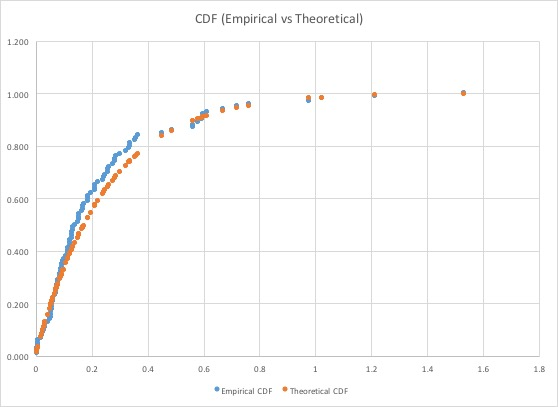
\includegraphics[scale = 0.45]{Picture2.jpg}
\end{center}
They pretty much match with one another. The reason is that because the 100 random numbers are exponentially distributed as indicated in the problem. The more generated random numbers, the closer the curve fits the exponential CDF.
\item
First, we find the end time in seconds for each query.  Then, we set up the histogram table for each-second interval to account for the number of queries being served during that interval. Last, we plot the normalized histogram (number of queries divided by the total 100 queries).\\
\begin{center}
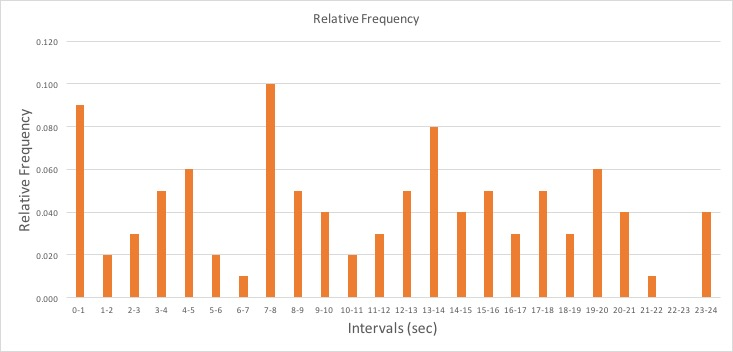
\includegraphics[scale = 0.5]{Picture3.jpg}
\end{center}
From intuition plus eyeballing, it is concluded that the distribution is Poisson as we assumed the "random" inter-arrival times.\\
The formula is written as below:\\
\begin{equation}
f(x) = \left(\frac{4^x}{x!}\right)e^{-4}
\end{equation}
\end{enumerate}

\section*{Problem 4}
\begin{enumerate}[(a)]
\item
Assume the four-level cache system is M/M/1 and 
Given:\\
$Pr(X_{1} = Hit) = \frac{1}{2}, Pr(X_{2} = Hit) = \frac{3}{5}, Pr(X_{3} = Hit) = \frac{7}{10}$ for L1, L2 and L3 cache\\
then we can derive the following:
$\text{Probability of L1 hit} = Pr(X_{1} = Hit) = 0.5$\\
$\text{Probability of L2 hit after L1 miss} = Pr(X_{1} = Miss)*Pr(X_{2} = Hit)= 0.5*0.6 = 0.3$\\
$\text{Probability of L3 hit after L2 miss} = Pr(X_{1} = Miss)*Pr(X_{2} = Miss)*Pr(X_{3} = Hit) = 0.5*0.4*0.7 = 0.14$\\
$\text{Probability of accessing the last memory level} = Hit | \bar X_{1}\cap \bar X_{2}\cap \bar X_{3}) = \frac{1}{2}*\frac{2}{5}*\frac{3}{10} = \frac{3}{50}$\\
$T(L1)_s = 1, T(L2)_s = 2, T(L3)_s = 7, T(rest)_s = 20 $\\
so PMF for random variable $t$ is:\\
\begin{equation}
  f(t) =\left\{
  \begin{array}{@{}ll@{}ll@{}ll@{}}
    0.5, & t =1 \\
    0.3, & t = 3 \\
    0.14, & t = 10 \\
    0.06, & t = 30
  \end{array}\right.
\end{equation} 
\item
$\mu = \mathds{E}(t) = (0.5)1 + (0.3)3 + (0.14)10 + (.06)30 = 4.6 \text{   clock cycles}$
\item
$$variance = \sum_{i = 1}^4 [(x_i -\mu)^2p_i] = 0.5(4.6 - 1)^2 + 0.3(4.6 - 3)^2 + 0.14(4.6 - 10)^2 + 0.06(4.6 - 30)^2 = 50.04$$
so the standard deviation for random variable $t$ is $\sqrt(50.04) = 7.07  \text{   clock cycles}$\\
\item

\end{enumerate}

\section*{Problem 5}
\begin{enumerate}[(a)]
\item
By comparing both the empirical cdf and theoretical cdf (by finding the differences between the range/bin defined in the table, see excel), one can conclude both are similar and match to each other. As the central limit theorem states: the arithmetic mean of 100 independent random variables (which has the mean and variance defined to be uniformally distributed) will be normally distributed. This exercise just proves CLT.\\
\begin{center}
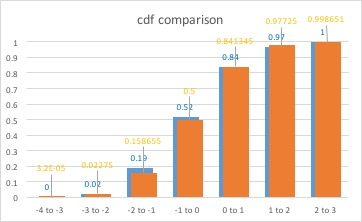
\includegraphics{Picture1.jpg}
\end{center}
\item

\end{enumerate}

\end{document}